\documentclass[conference]{IEEEtran}
\usepackage[utf8]{inputenc}
\usepackage[croatian]{babel}
\usepackage{amsmath}
\usepackage{amsfonts}
\usepackage{comment}
\usepackage{amssymb}
\usepackage{graphicx}
\usepackage{hyperref}
\usepackage{listings}
\usepackage{caption}
\usepackage{amsmath}
\usepackage{float}

\hyphenation{op-tical net-works semi-conduc-tor}

\begin{document}

\title{Analiza stava u filmskim kritikama}

%5-10 stranica
%uvod (motivacija i ciljevi), opis problema (skup podataka), opis vaše metode i pristupa za rješavanje problema, prikaz rezultata (grafovi), osvrt na druge pristupe, mogući budući nastavak istraživanja

\author{
	\IEEEauthorblockN{Antonio Kovačić}
	\IEEEauthorblockA{
		Sveučilište u Zagrebu\\
    	PMF--Matematički odsjek\\
    	Računarstvo i matematika\\
    	Zagreb, Hrvatska\\
    	in.math0@gmail.com
	}
	\and
	\IEEEauthorblockN{Janko Marohnić}
	\IEEEauthorblockA{
		Sveučilište u Zagrebu\\
    	PMF--Matematički odsjek\\
    	Računarstvo i matematika\\
    	Zagreb, Hrvatska\\
    	janko.marohnic@gmail.com
	}
	\and
	\IEEEauthorblockN{Lana Arzon}
	\IEEEauthorblockA{
		Sveučilište u Zagrebu\\
    	PMF--Matematički odsjek\\
    	Računarstvo i matematika\\
    	Zagreb, Hrvatska\\
    	lana.arzon@gmail.com
	}
}

\maketitle

\begin{abstract}
Analiza stava (\textit{Sentiment Analysis}) je problem klasifikacije teksta čiji je cilj odrediti stav autora teksta o temi koja je obrađena u tom tekstu. U najjednostavnijem obliku, određuje se da li je stav pozitivan ili negativan. U ovom istraživanju ćemo se baviti analizom stava u filmskim kritikama, odnosno određivanjem da li je kritika pozitivna ili negativna. Koristit ćemo različite metode odabira značajki i dvije poznate metode za klasifikaciju teksta -- Naive Bayes i SVM, te napraviti usporedbu njihovih uspješnosti u različitim kombinacijama.
\end{abstract}

\IEEEpeerreviewmaketitle

\section{Uvod}

Analiza stava jedan je od zadataka prirodne obrade teksta (\textit{Natural Language Processing} -- NLP), grane računarstva, umjetne inteligencije i lingvistike koja se bavi interakcijama između računala i ljudskog (prirodnog) jezika. Jedan od glavnih izazova u NLP je omogućiti računalima "razumijevanje" prirodnog jezika, to jest omogućiti im obradu teksta napisanog prirodnim jezikom u svrhu automatskog generiranja željenih rezultata. Današnji NLP algoritmi koriste metode strojnog učenja, najčešće statističke metode. Sljedeće tri metode pokazale su se vrlo efikasnim kod rješavanja problema klasične klasifikacije teksta po temi: Naive Bayes, metoda maksimalne entropije (\textit{Maximum Entropy}) i metoda potpornih vektora (\textit{Support Vector Machines} -- SVM). Analiza stava pokazala se nešto zahtjevnijim (ali i izazovnijim) zadatkom pa ne očekujemo tako dobre rezultate. Naime, ono što analizu stava čini teškom je to da stav nije samo zbroj sentimentalne vrijednosti riječi već ovisi i o kontekstu, a i često se izražava neizravno. Ipak, ove standardne metode trebale bi dati zadovoljavajuće rezultate pa ćemo dvije od navedenih iskoristiti u našem istraživanju: Naive Bayes i SVM.

\section{Opis problema}

Cilj ovog istraživanja je otkriti da li je stav nekog teksta pozitivan ili negativan, to jest naučiti klasifikator da što bolje (točnije) raspoređuje tekstove na ove dvije klase. Konkretno, bavimo se pitanjem da li je filmska kritika pozitivna ili negativna. Koristit ćemo skup podataka "Movie Review Data" \cite{dataset}, točnije polarity dataset, koji je sastoji od ukupno 2000 tekstova filmskih kritika pisanih na engleskom jeziku, 1000 pozitivnih i 1000 negativnih. Pomoću ovog skupa podataka i metoda strojnog učenja omogućit ćemo da klasifikator određuje i stav novih kritika (na kojima nije treniran).

\section{Alati}

\subsection{NLTK}

NLTK (\textit{Natural Language Toolkit}) je niz biblioteka i programa za simboličko i statističko obrađivanje podataka pomoću programskog jezika Pythona. NLTK uključuje grafičko prikazane ogledne primjerke te je popraćen opsežnom dokumentacijom i uključuje knjigu \cite{nltk} objašnjenja fundamentalnih načela zadataka podržanih od strane ovog alata.

NLTK je pretežito namjenjen učenju o računalnoj obradi prirodnog jezika ili pak za istraživanja u obradi prirodnog jezika i sličnih bliskih struka poput empirijske lingvistike, kognitivnih znanosti, umjetne inteligencije, vađenju informacija (iz dokumenata) i strojnom učenju. Mi smo ovaj alat iskoristili za pretvaranje tekstova kritika u liste riječi (tokenizacija) te za klasifikaciju pomoću Naive Bayes klasifikatora.

\subsection{scikit-learn}

scikit-learn je open source biblioteka za strojno učenje pomoću programskog jezika Python. Sadrži različite algoritme za klasifikaciju, regresiju i klasteriranje uključujući SVM, logističku regresiju, Naive Bayes algoritam, k-means i mnoge druge. Ova biblioteka povezana je s numeričkim i znanstvenim Python bibliotekama NumPy i SciPy. Mi smo je koristili kod klasifikacije metodom potpornih vektora (SVM).

\subsection{Matlab}
Za crtanje grafova - bar dijagrama i linijskih grafova koristili smo Matlab programski paket. Crtanje tih dijagrama nam pomaže da shvatimo odnos točnosti među različitim modelima.

\section{Odabir značajki}

Značajke (\textit{features}) su karakteristike teksta pomoću kojih metoda nastoji dobiti sliku o tome koji stav dominira u tekstu. Odabir značajki vrlo je važan proces jer bitno utječe na brzinu i kvalitetu klasifikacije. Potrebno je odabrati one značajke koje će nam na neki način dati najviše informacije o stavu teksta pazeći pritom da ih ne odaberemo niti previše, a niti premalo. Odaberemo li previše značajki, učenje klasifikatora može trajati jako dugo, a postoji i opasnost od pretreniranja (overfitting). S druge strane, premali broj značajki sigurno neće dati zadovoljavajuću klasifikaciju na novim primjerima, a mogući je čak i underfitting.

Kao značajke ćemo koristiti prvenstveno riječi iz liste odabranih sentiment riječi \cite{words} koje su se pokazale kao dobar indikator stava u filmskim kritikama. Ovaj skup sadrži oko 6800 riječi. Samo ovakvim jednostavnim pristupom uspjeli smo postići zadovoljavajuću točnost (oko $80\%$ za sve metode uz male varijacije). No, učenje klasifikatora je relativno sporo zbog prevelikog broja značajki. Ipak, zbog dobrog rezultata klasifikacije, daljnji odabir značajki ćemo raditi na temelju ove liste riječi.

Kod analize kritika služit ćemo se jednostavnom metodom "bag of words" koja se temelji samo na pojavljivanju (prisutstvu ili frekvenciji) značajke u tekstu, ne uzimajući u obzir poredak i vezu s ostalim značajkama. Dakle, pretpostavljamo da su značajke nezavisne.

\subsection{Najveća frekvencija}

Jedna od najjednostavnijih metoda odabira značajki je promatranje frekvencije potencijalne značajke u skupu za učenje. Za svaku riječ ćemo izračunati njenu apsolutnu frekvenciju (ukupan broj pojavljivanja) u svim kritikama iz korištenog skupa za učenje. Riječi ćemo zatim sortirati silazno po frekvenciji te prvih 1000 koristiti kao značajke u metodama klasifikacije. Iako je vrlo jednostavna, ova metoda je dala iznenađujuće dobre rezultate (oko $80\%$).

\subsection{TF-IDF}

TF-IDF (\textit{Term Frequency, Inverse Document Frequency}) je način vrednovanja važnosti neke riječi u dokumentu temeljen na tome koliko se često ta riječ pojavljuje u danom skupu dokumenata. Ako se riječ pojavljuje često u dokumentu, ona je važna te ćemo joj dodijeliti visoki rezultat. No, ako se riječ pojavljuje u velikom broju dokumenata, ona vjerojatno neće biti dobar indikator stava pa ćemo joj dodijeliti mali rezultat. Za svaku riječ proći ćemo po svim kritikama i izračunati pripadni TF-IDF te zapamtiti maksimalnu vrijednost. Spremit ćemo 1000 riječi s najvećom maksimalnom TF-IDF vrijedošću te ih kasnije koristiti kao značajke kod klasifikacije. Ova metoda se nije pokazala dobrom jer je smanjila točnost modela (na oko $70\%$).

\subsection{Najinformativnije značajke Naive Bayes klasifikatora}

Ova metoda odabira značajki koristi Naive Bayes klasifikator implementiran u alatu NLTK. Najprije smo naučili klasifikator na svim riječima iz prethodno spomenute liste te zatim spremili 500 riječi koje je klasifikator ocijenio kao najinformativnije (most\_infotmative\_features). Nakon što smo pokrenuli novi Naive Bayes klasifikator koji kao značajke koristi samo ovih 500 riječi primijetili smo poboljšanje i u brzini učenja, ali i u točnosti (oko $85\%$).

\begin{figure}[H]
\begin{minipage}{0.5\textwidth}
\centering
\begin{lstlisting}[language = Python, frame = single, basicstyle=\tiny\ttfamily, xleftmargin = 5pt, xrightmargin = 5pt]
>>> classifier.show_most_informative_features(10)
Most Informative Features
               insulting = True           negati : positi =     16.9 : 1.0
               ludicrous = True           negati : positi =     12.5 : 1.0
               strongest = True           positi : negati =     11.8 : 1.0
             outstanding = True           positi : negati =     11.5 : 1.0
               stupidity = True           negati : positi =     11.3 : 1.0
              astounding = True           positi : negati =     11.1 : 1.0
               laughably = True           negati : positi =     10.9 : 1.0
                 idiotic = True           negati : positi =     10.5 : 1.0
                  hatred = True           positi : negati =     10.4 : 1.0
        incomprehensible = True           negati : positi =      8.9 : 1.0
\end{lstlisting}
\caption{Najinformativnije značajke i njihov "likelihood ratio"}
\end{minipage}
\end{figure}

\section{Metode strojnog učenja}

\subsection{Naive Bayes}

Naive Bayes je jednostavna metoda strojnog učenja koja se temelji na Bayesovom pravilu primijenom na dokument $d$ i klasu $c$:

\[P(c|d) = \frac{P(d|c)P(c)}{P(d)}.\]

Klasa kojoj najvjerojatnije pripada dokument (maximum a posteriori class) dana je s:

\[c_{\text{MAP}} = \underset{{c \in C}}{\text{argmax }} \frac{P(d|c)P(c)}{P(d)}
= \underset{{c \in C}}{\text{argmax }} P(d|c)P(c).\] 

Odnosno, ako dokument $d$ reprezentiramo pomoću značajki $x_1, x_2, \ldots, x_n$:

\[c_{\text{MAP}} = \underset{{c \in C}}{\text{argmax }} P(x_1, x_2, \ldots, x_n|c)P(c).\]

Osnovna pretpostavka koju koristi Naive Bayes je da su značajke međusobno nezavisne, to jest da vrijedi:

\[P(x_1, x_2, \ldots, x_n|c) = \prod_{i=1}^n P(x_i|c).\]

Ova pretpostavka uvodi se zbog brzine i jednostavnijeg računanja. Iako je ona očito pogrešna, Naive Bayes se pokazao kao jako dobra metoda za klasifikaciju teksta, pa tako i za analizu stava. U našem slučaju (analiza stava u filmskim kritikama), uz dobar odabir značajki, daje također zadovoljavajuće rezultate (u najboljem slučaju uspjeli smo postići točnost od $87.2\%$ na skupu za testiranje).

\subsection{SVM}

Metoda potpornih vektora (SVM) je skup metoda za nadzirano učenje korišten za
klasifikaciju, regresiju i detekciju \textit{outlier}-a.

Prednosti metode potpornih vektora su nad Naivnim Bayesom su:

\begin{itemize}
  \item efikasan kod više featurea
  \item koristi samo podskup skupa za treniranje (tzv. potporni vektori), pa je
    memorijski efikasan
  \item prilagodljiv: možemo koristiti više \textit{kernela} za funkciju izbora
\end{itemize}

Mane metode potpornih vektora su:

\begin{itemize}
  \item ako je broj značajki puno veći od broja uzoraka, onda metoda vjerojatno
    neće davati dobre rezultate
  \item potproni vektori ne daju direktno vjerojatnosne procjene, one se računaju
    (skupom) 5-strukom unakrsnom validacijom
\end{itemize}

Postoje tri poznate vrste kernela koje se koriste: Linearni, polinomijalni i
RBF\footnote{eng. \textit{Radial basis function}, funkcija koja ovisi samo o
udaljenosti od neke točke, tzv. \textit{radijalna} funkcija}. Od ova 3 kernela,
Linearni i polinomijalni su nam dobro funkcionirali.

SVM ima veliki broj parametara kojima možemo specificirati točno kako želimo
da naš algoritam radi. Mi smo koristili sljedeće parametre (i
neke varirali, te ćemo navesti one koje daju najbolji rezultat u zadnjem
poglavlju):

\begin{itemize}
  \item{\textbf{C}:} Dopuštena greška
  \item{\textbf{kernel}:} Može biti ``linear", ``poly", ``rbf" i ``sigmoid".
  \item{\textbf{degree}:} Kada koristimo polinomijalni kernel, onda ova opcija
    specificira stupanj polinoma
  \item{\textbf{gamma}:} Koeficijent kernela
  \item{\textbf{tol}:} Tolerancija konvergiranja, u kojem trenutku će algoritam
    stati
\end{itemize}

\section{Evaluacija}

Imali smo 4 različita izbora značajki, s kojima smo trenirali i evaluirali
naše modele:

\begin{enumerate}
  \item Lista sentiment riječi (oko 6800 riječi)
  \item Riječi s najvećom frekvencijom (1000 riječi)
  \item Riječi s najvećom maksimalnom TF-IDF vrijednošću (1000 riječi)
  \item Najinformativnije značajke Naive Bayes klasifikatora (500 riječi)
\end{enumerate}

Za provjeru modela i izbor parametera koristili smo k-struku unakrsnu
validaciju. Provjerili smo kako izbor $k$ utječe na točnost klasifikatora,
i nije bilo neke znatne razlike, pa smo uzeli $k = 5$.

\begin{figure}[H]
\begin{minipage}{0.5\textwidth}
\centering
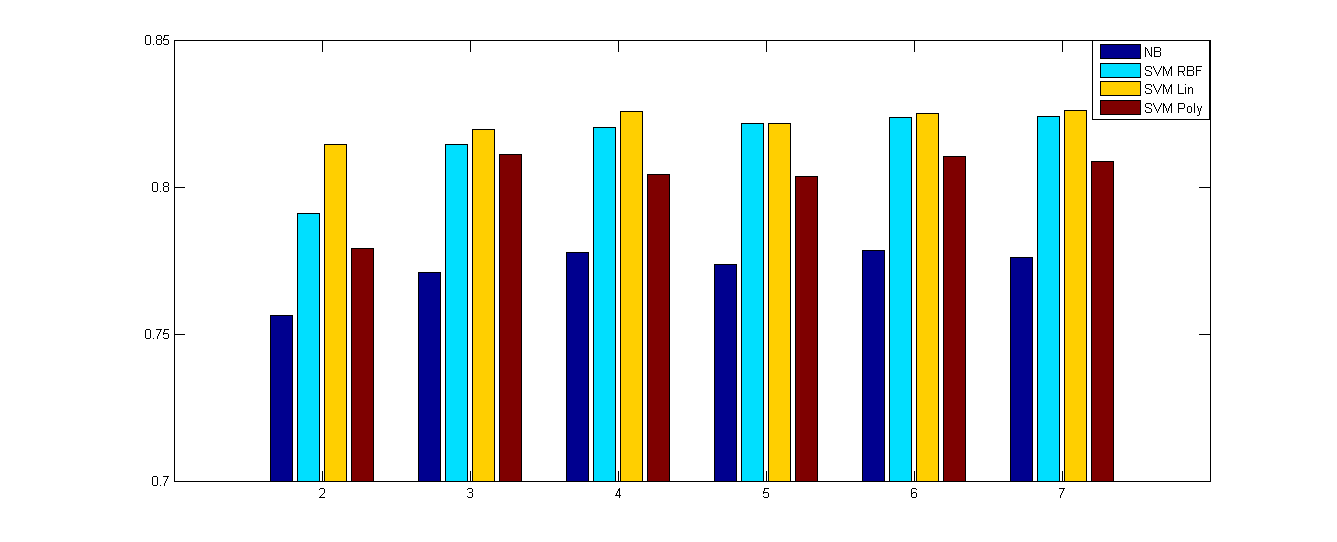
\includegraphics[width=\textwidth]{images/testK-fold.png}
\caption{Mjerenje točnosti za razne indekse $k$ u $k$-strukoj unakrsnoj validaciji-značajke čini lista sentimenta riječi}
\end{minipage}
\end{figure}

Veličina skupa za unakrsnu validaciju je 1500 kritika. Na kraju testiramo
model tako da uzmemo taj skup od 1500 kritika kao skup za treniranje, a onda
uzmemo još 500 novih kritika kao skup za testiranje.

Za mjeru koliko je neki klasifikator "dobar", korstili smo prosječnu
\textit{točnost} kod 5-struke unakrsne validacije. Razlog zašto nismo uzeli
$F_1$ mjeru je taj što mi na svojem skupu imamo jednaki broj pozitivnih i
negativnih kritika. $F_1$ dobro ocjenjuje tzv. \textit{precision} i
\textit{recall}, koje trebamo promatrati u slučaju kada imamo puno veći broj
jedne vrste kritika nego druge, što kod nas nije slučaj.

U nastavku navodimo izbor značajki za svaki klasifikator, i parametre za SVM
i njegove varijante. U sekciji "Rezultati" ćemo zatim navesti koji izbor
parametara je bio najbolji, i koja je bila točnost svakog klasifikatora na
testnom skupu.

\subsection{Naive Bayes}

Kod izbora značajki, najbolje rezultate za Naive Bayes dobili smo
kada smo za značajke koristili najinformativnije značajke Naive Bayes
klasifikatora (koji je korišten samo u svhru odabira značajki, na njemu nismo
testirali).

\subsection{SVM}

Kod izbora značajki, najbolji rezultat za SVM smo dobili kod izbora liste
sentiment riječi.

Općenito smo varirali parametre $C$, $\gamma$ i $degree$, na sljedećim skupovima:

\begin{itemize}
  \item $C \in \{0 + i \cdot 0.01 | i = 1,\ldots,100\}$
  \item $\gamma \in \{2^i| i \in \mathbb{Z}, -6 \leq i <6 \}$ (grafove smo
    prikazivali logaritamskom skalom)
  \item $degree \in \{2,3,4\}$ ($degree = 1$ je zapravo linerani kernel)
\end{itemize}

\subsubsection{RBF kernel}

Varirali $C$ i $\gamma$, i dobili smo sljedeća mjerenja za točnost:

\begin{figure}[H]
\begin{minipage}{0.5\textwidth}
\centering
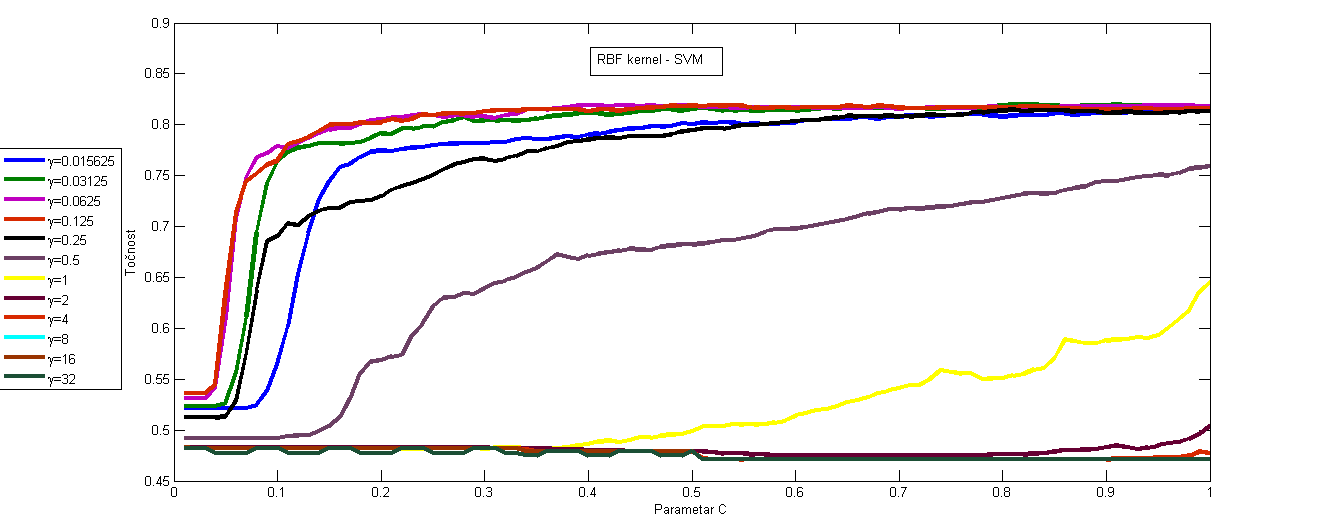
\includegraphics[width=\textwidth]{images/allRBF.png}
\caption{Graf $C$/točnost za SVM s RBF-om}
\end{minipage}
\end{figure}

\subsubsection{Linearni kernel}

Varirali smo $C$, i dobili smo sljedeća mjerenja za točnost:

\begin{figure}[H]
\begin{minipage}{0.5\textwidth}
\centering
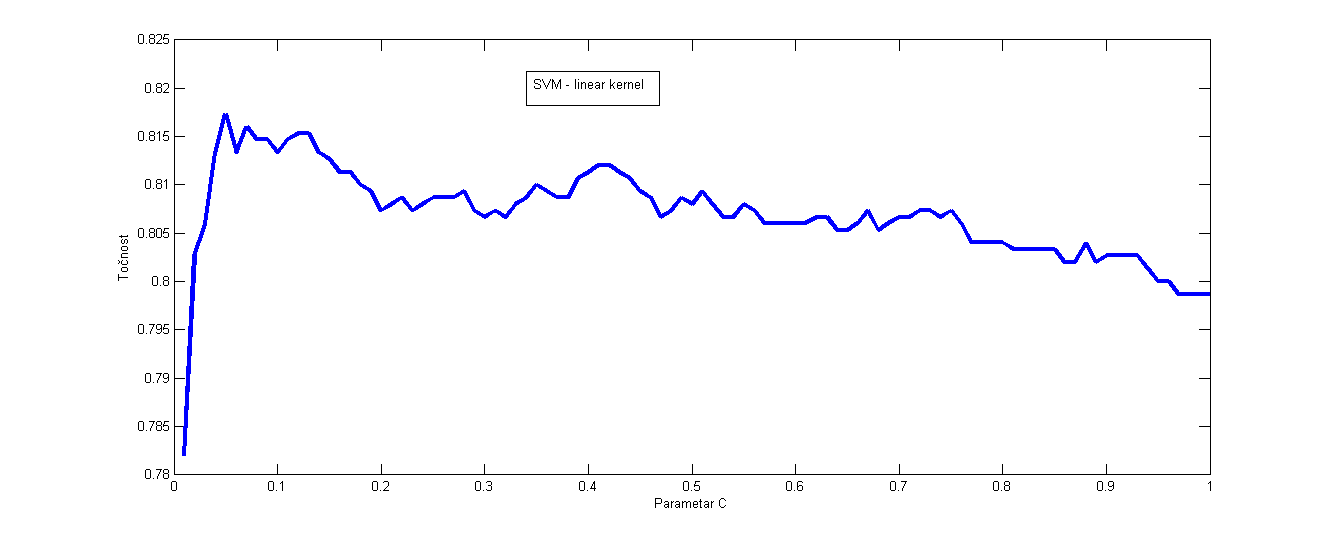
\includegraphics[width=\textwidth]{images/paraCLinear.png}
\caption{Graf $C$/točnost za SVM s linearnim kernelom}
\end{minipage}
\end{figure}

\subsubsection{Polinomijalni kernel}

Varirali smo $C$, $\gamma$ i $degree$, i dobili smo sljedeća mjerenja za točnost:

\begin{figure}[H]
\begin{minipage}{0.5\textwidth}
\centering
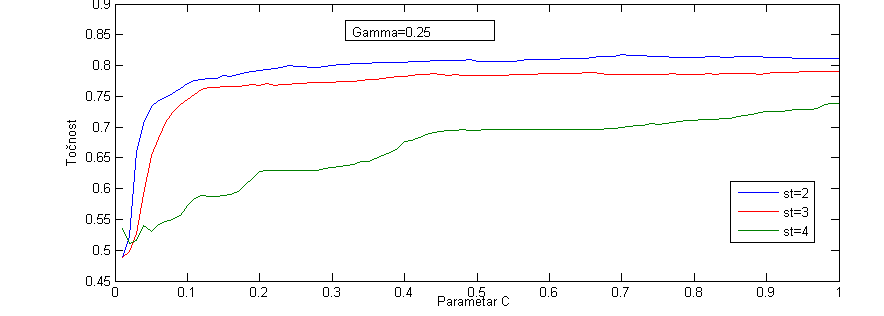
\includegraphics[width=\textwidth]{images/paramCPoly.png}
\caption{Graf C/točnost za SVM s polinomijalnim kernelom}
\end{minipage}
\end{figure}

\begin{figure}[H]
\begin{minipage}{0.5\textwidth}
\centering
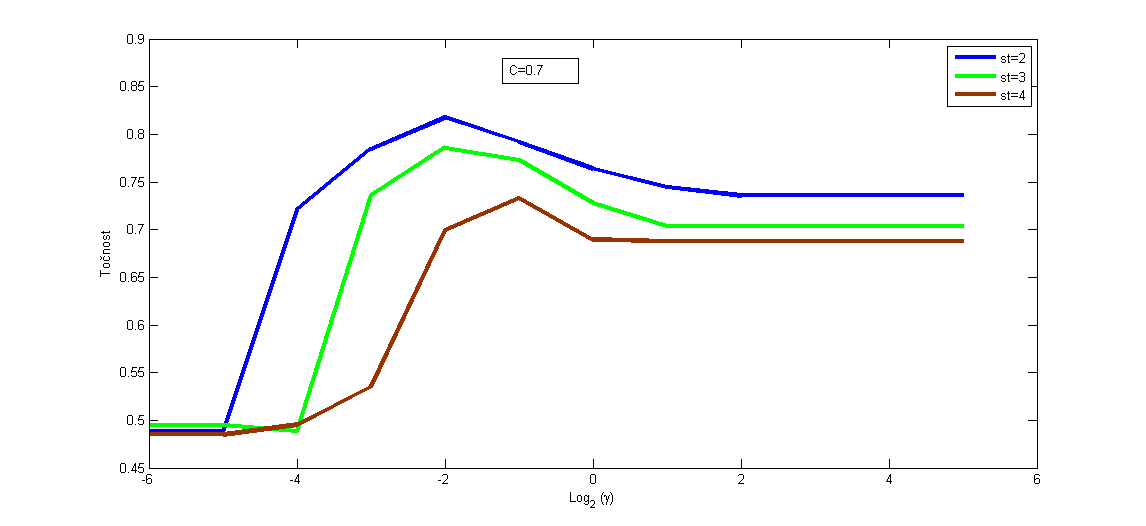
\includegraphics[width=\textwidth]{images/paramGammaPoly.png}
\caption{Graf $\log _2(\gamma )$/točnost za SVM s polinomijalnim kernelom}
\end{minipage}
\end{figure}

\begin{figure}[H]
\begin{minipage}{0.5\textwidth}
\centering
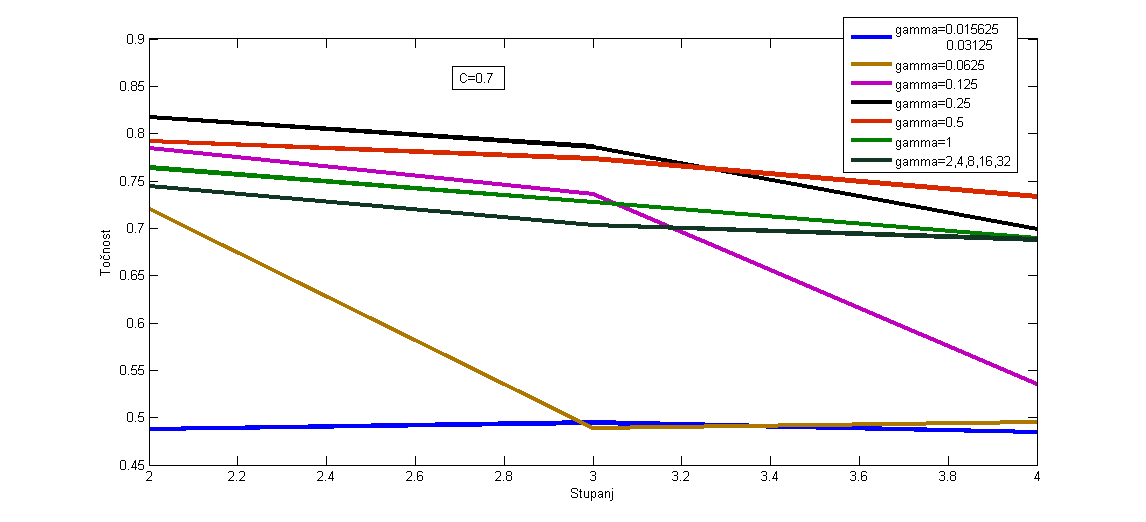
\includegraphics[width=\textwidth]{images/paramDegreePoly.png}
\caption{Graf Stupanj/točnost za SVM s polinomijalnim kernelom}
\end{minipage}
\end{figure}

\section{Rezultati}

Optimalni parametri za SVM (oni koji imaju najveću točnost u unakrsnoj
validaciji) ispali su sljedeći:

\begin{itemize}
  \item RBF kernel: $C=0.91, \gamma =0.03125$
  \item Linearni kernel: $C=0.05$
  \item Polinomijalni kernel: $C=0.7, \gamma =0.25, degree=2$
\end{itemize}

Sljedeći graf prikazuje konačni rezultat našeg istraživanja, odnosno prikazuje
usporedbu sva 4 klasifikatora na testnom skupu (novom skupu kojeg nismo
koristili u unakrsnoj validaciji)

\begin{figure}[H]
\begin{minipage}{0.5\textwidth}
\centering
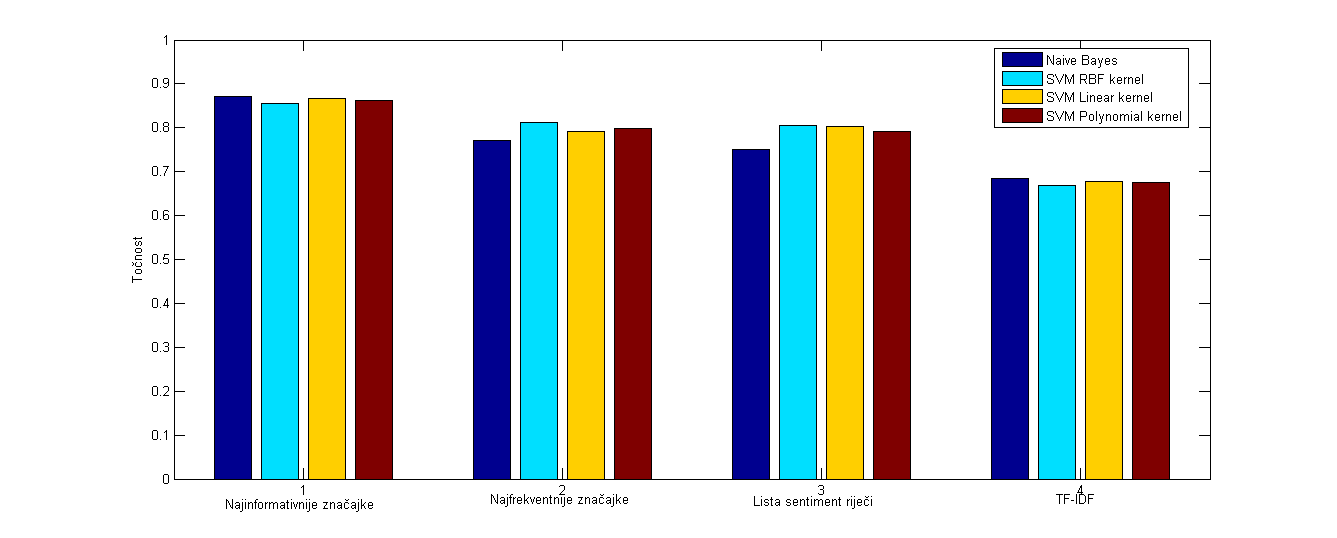
\includegraphics[width=\textwidth]{images/SVM_tocnost.png}
\caption{Točnost Naive Bayes (tamno plavo) \& SVM RBF (svjetlo plavo) \& SVM Linear (žuto) \& SVM Polynomial (crveno)}
\end{minipage}
\end{figure}

Navodimo i konfuzijske matrice svakog klasifikatora na istom testnom skupu.

\begin{figure}[H]
\begin{minipage}{0.5\textwidth}
\centering
\begin{tabular}{|c|c|c|c|}
  \hline
  \multicolumn{2}{|c|}{Matrica}  & \multicolumn{2}{|c|}{Stvarna klasa} \\ 
  \cline{3-4}
  \multicolumn{2}{|c|}{konfuzije} & pozitivno & negativno \\ 
  \hline
  Predviđeno & pozitivno & 224 & 34 \\
  \cline{2-4}
  modelom & negativno & 38 & 204 \\
  \hline
\end{tabular}
\caption{Matrica konfuzije za Naive Bayes metodu uz odabir značajki pomoću najinformativnijih značajki (točnost $85.6\%$)}
\end{minipage}
\end{figure}

\begin{figure}[H]
\begin{minipage}{0.5\textwidth}
\centering
\begin{tabular}{|c|c|c|c|}
  \hline
  \multicolumn{2}{|c|}{Matrica}  & \multicolumn{2}{|c|}{Stvarna klasa} \\ 
  \cline{3-4}
  \multicolumn{2}{|c|}{konfuzije} & pozitivno & negativno \\ 
  \hline
  Predviđeno & pozitivno & 217 & 61 \\
  \cline{2-4}
  modelom & negativno & 37 & 185 \\
  \hline
\end{tabular}
\caption{Matrica konfuzije za SVM (linearni kernel) (točnost $82\%$) uz odabir značajki koje su najinformativnije}
\end{minipage}
\end{figure}

\begin{figure}[H]
\begin{minipage}{0.5\textwidth}
\centering
\begin{tabular}{|c|c|c|c|}
  \hline
  \multicolumn{2}{|c|}{Matrica}  & \multicolumn{2}{|c|}{Stvarna klasa} \\ 
  \cline{3-4}
  \multicolumn{2}{|c|}{konfuzije} & pozitivno & negativno \\ 
  \hline
  Predviđeno & pozitivno & 214 & 56 \\
  \cline{2-4}
  modelom & negativno & 40 & 190 \\
  \hline
\end{tabular}
\caption{Matrica konfuzije za SVM (polinomni kernel) (točnost $82\%$) uz odabir značajki koje su najinformativnije}
\end{minipage}
\end{figure}

\begin{figure}[H]
\begin{minipage}{0.5\textwidth}
\centering
\begin{tabular}{|c|c|c|c|}
  \hline
  \multicolumn{2}{|c|}{Matrica}  & \multicolumn{2}{|c|}{Stvarna klasa} \\ 
  \cline{3-4}
  \multicolumn{2}{|c|}{konfuzije} & pozitivno & negativno \\ 
  \hline
  Predviđeno & pozitivno & 217 & 58 \\
  \cline{2-4}
  modelom & negativno & 37 & 188 \\
  \hline
\end{tabular}
\caption{Matrica konfuzije za SVM (RBF) (točnost $82\%$) uz odabir značajki koje su najinformativnije}
\end{minipage}
\end{figure}

\section{Zaključak}

U konačnosti možemo reći da se naši rezultati djelomično poklapaju s
očekivanjima. Metoda potpornih vektora u globalu daje neznatno bolje rezultate.
Naive Bayes daje bolje rezultate kada smo kao metodu za izbor značajki odabrali
najinformativnije riječi. Procjenjena greška koja se događa na testnom skupu
ispada u prosjeku oko $17\%$ za odabir značajki različit od $tf-idf$, inače
prosječna greška ispada oko $30\%$.

\begin{thebibliography}{1}

\bibitem{thumbsup}
	B. Pang, L. Lee, S. Vaithyanathan,
 	Thumbs Up?: Sentiment Classification Using Machine Learning Techniques,
 	Proceedings of the ACL-02 Conference on Empirical Methods in Natural Language Processing - Volume 10,
 	Association for Computational Linguistics,
	Stroudsburg, PA, USA,
	2002.
	
\bibitem{stan}
	S. Jain, S. Nayak,
	Sentiment Analysis of Movie Reviews: A Study of Features and Classifiers\\
	\url{http://www.stanford.edu/~nayaks/reportsFolder/cs221_report.pdf}
	
\bibitem{uupp}
	M. Božić, I. Gavran,
	Analiza stava\\
	\url{http://stav.math.hr/static/data/uupp.pdf}
	
\bibitem{nltk}
	S. Bird, E. Klein, E. Loper,
	Natural Language Processing with Python,
	O'Reilly Media,
	2009.
	
\bibitem{tfidftutorial}
	S. Loria,
	Tutorial: Finding Important Words in Text Using TF-IDF\\
	\url{http://stevenloria.com/finding-important-words-in-a-document-using-tf-idf/}

\bibitem{dataset}
	B. Pang, L. Lee,
	Movie Review Data\\
	\url{https://www.cs.cornell.edu/people/pabo/movie-review-data/}
	
\bibitem{words}
	Opinion Lexicon (Sentiment Lexicon)\\
	\url{http://www.cs.uic.edu/~liub/FBS/sentiment-analysis.html#lexicon}
	
\bibitem{githubrepo}
	A. Kovačić, J. Marohnić, L. Arzon,
	Analiza stava u filmskim kritikama,
	GitHub repozitorij\\
	\url{https://github.com/janko-m/college-machine_learning}

\bibitem{scikit}
    Scikit-learn developeri,
    Support Vector Machines\\
    \url{http://scikit-learn.org/stable/modules/svm.html}

\end{thebibliography}

\end{document}
